\documentclass{amsart}
\usepackage[margin = 2.5cm]{geometry}
\usepackage{sagetex} % Para usar sagetex
%\usepackage[usefamily=sage]{pythontex} % Para usar pythontex
\usepackage[utf8]{inputenc}
\usepackage{tikz}

\newtheorem{ejer}{Ejercicio}

\title{Álgebra y Matemática Discreta. GII - FIUM. \\ Parcial 1}
\begin{document}
\maketitle


\begin{ejer} 
Calcula el determinante de la siguiente matriz sobre el cuerpo
${\mathbb Z}_5$ realizando operaciones elementales. 
$$ \left|\begin{array}{rrrr}
1 & 0 & 2 & 0 \\
3 & 3 & 2 & 0 \\
3 & 4 & 0 & 4 \\
0 & 2 & 4 & 3
\end{array}\right|$$
{\bf Este problema hay que hacerlo a mano en el papel proporcionado
en el examen.}
\end{ejer}

{\it Solución: }

$$
\left|\begin{array}{rrrr}
	1 & 0 & 2 & 0 \\
	3 & 3 & 2 & 0 \\
	3 & 4 & 0 & 4 \\
	0 & 2 & 4 & 3
\end{array}\right| 
\to E_{(3) - 3(1)}
\left|\begin{array}{rrrr}
	1 & 0 & 2  & 0 \\
	3 & 3 & 2  & 0 \\
	0 & 4 & 4 & 4 \\
	0 & 2 & 4  & 3
\end{array}\right| 
\to E_{(2) - 3(1)}
\left|\begin{array}{rrrr}
	1 & 0 & 2  & 0 \\
	0 & 3 & 1  & 0 \\
	0 & 4 & 4  & 4 \\
	0 & 2 & 4  & 3
\end{array}\right| 
\to E_{(3) - 2(4)}
\left|\begin{array}{rrrr}
	1 & 0 & 2 & 0 \\
	0 & 3 & 1 & 0 \\
	0 & 0 & 1 & 3 \\
	0 & 2 & 4 & 3
\end{array}\right|
$$
$$
\to E_{(2) - (4)}
\left|\begin{array}{rrrr}
	1 & 0 & 2 & 0 \\
	0 & 1 & 2 & 2 \\
	0 & 0 & 1 & 3 \\
	0 & 2 & 4 & 3
\end{array}\right| 
\to E_{(1) - 2(3)}
\left|\begin{array}{rrrr}
	1 & 0 & 0 & 4 \\
	0 & 1 & 2 & 2 \\
	0 & 0 & 1 & 3 \\
	0 & 2 & 4 & 3
\end{array}\right| 
\to E_{(2) - 2(3)}
\left|\begin{array}{rrrr}
	1 & 0 & 0 & 4 \\
	0 & 1 & 0 & 1 \\
	0 & 0 & 1 & 3 \\
	0 & 2 & 4 & 3
\end{array}\right| 
\to E_{(1) - (4)}
\left|\begin{array}{rrrr}
	1 & 0 & 0 & 0 \\
	0 & 1 & 0 & 1 \\
	0 & 0 & 1 & 3 \\
	0 & 2 & 4 & 3
\end{array}\right| 
$$
$$
\to E_{(4) - 2(2)}
\left|\begin{array}{rrrr}
	1 & 0 & 0 & 0 \\
	0 & 1 & 0 & 1 \\
	0 & 0 & 1 & 3 \\
	0 & 0 & 4 & 1
\end{array}\right|
\to E_{(4) - 4(3)}
\left|\begin{array}{rrrr}
	1 & 0 & 0 & 0 \\
	0 & 1 & 0 & 1 \\
	0 & 0 & 1 & 3 \\
	0 & 0 & 0 & 4
\end{array}\right|
\to E_{4(4)} 4
\left|\begin{array}{rrrr}
	1 & 0 & 0 & 0 \\
	0 & 1 & 0 & 1 \\
	0 & 0 & 1 & 3 \\
	0 & 0 & 0 & 1
\end{array}\right|
\to E_{(3) - 3(4)} 4
\left|\begin{array}{rrrr}
	1 & 0 & 0 & 0 \\
	0 & 1 & 0 & 1 \\
	0 & 0 & 1 & 0 \\
	0 & 0 & 0 & 1
\end{array}\right|
$$
$$
\to E_{(2) - (4)} 4
\left|\begin{array}{rrrr}
	1 & 0 & 0 & 0 \\
	0 & 1 & 0 & 1 \\
	0 & 0 & 1 & 0 \\
	0 & 0 & 0 & 1
\end{array}\right|
\to E_{(2) - (4)} 4
\left|\begin{array}{rrrr}
	1 & 0 & 0 & 0 \\
	0 & 1 & 0 & 0 \\
	0 & 0 & 1 & 0 \\
	0 & 0 & 0 & 1
\end{array}\right|
= 4 |I| = 4
$$

\pagebreak

\begin{ejer}
Encuentra todos los valores enteros $n$ que cumplan 
simultáneamente las siguientes condiciones:
\begin{align*}
n & \equiv 1 \pmod{25} \\
n & \equiv 52 \pmod{108} \\
n & \equiv 199 \pmod{201} 
\end{align*}
\end{ejer}

{\it Solución: }

% Escribe tu solución para el Ejercicio 2

\begin{align*}
	n &= 1 + 25x \\
	n &= 52 + 108y
\end{align*}

$$
	1 + 25x = 52 + 108y
$$
$$
	25x - 108y = 51
$$

$$
	\left[\begin{array}{c|cc}
		25  & 1 & 0      \\
		108 & 0 & 1      
	\end{array}\right]
	\to E_{(2) - 4(1)}
	\left[\begin{array}{c|cc}
		25  &  1 & 0      \\
		8   & -4 & 1      
	\end{array}\right]
	\to E_{(1) - 3(2)}
	\left[\begin{array}{c|cc}
		1  &  13 & -3      \\
		8  & -4  &  1      
	\end{array}\right]
	\to E_{(2) - 8(1)}
	\left[\begin{array}{c|cc}
		1  & -11  & -3      \\
		0  & -108 &  25     
	\end{array}\right]
$$

mcd(25, 108) = 1, tiene solución, caso 1

\begin{align*}
	25 \cdot (-11) + 108 \cdot (-3) &= 1 \\
	25 \cdot 84 + 108 \cdot 25 &= 0
\end{align*}

\begin{align*}
	25 \cdot (-11) \cdot 51 + 108 \cdot (-3) \cdot 51 &= 1 \\
	25 \cdot 84 t + 108 \cdot 25 t &= 0
\end{align*}

\begin{align*}
	x &= -561 + 84t \\
	y &= -153 + 25t
\end{align*}

Substituyendo la primera
$$
	n = 1 + 25 (-561 + 84t)
$$

$$
	n = -14025 + 2100t
$$

\begin{align*}
	n &\equiv -14025 \pmod{2100}
	n &\equiv -14025 \pmod{2100}
\end{align*}

% Fin del ejercicio 2

\pagebreak

\begin{ejer}
Sea $K = {\mathbb Z}_{43}$ y $f:K^4 \to K^3$ la aplicación lineal
dada por la matriz $$M(f) = \left(\begin{array}{rrrr}
24 & 23 & 11 & 26 \\
9 & 17 & 33 & 22 \\
16 & 16 & 13 & 4
\end{array}\right)$$
Encuentra dos aplicaciones lineales diferentes $g_1,g_2:K^3 \to K^4$ 
tales que $f\circ g_1 = {\sf id}_{K^3} = f\circ g_2$.
\end{ejer}

{\it Solución: }

% Escribe tu solución para el Ejercicio 3

\begin{sageblock}
	Mf = matrix(Zmod(43), [[24, 23, 11, 26], [9, 17, 33, 22], [16, 16, 13, 4]])
	Mftp = block_matrix([[Mf.T, 1]])
	Mftr = Mftp.echelon_form()
	Mftr = copy(Mftr)
	Mftr.subdivide([3], [3])
	g1 = Mftr.subdivision(0, 1).T
	
	T = column_matrix(Zmod(43), [1, 24, 14, 5])
	X = matrix(Zmod(43), [[0, 0, 1]])
	g2 = g1 + T * X
\end{sageblock}

Dos inversas por la derecha de $M(f)$, al no ser cuadrada hay infinitas
$$
	M(f) \cdot M(g_1) = I \to M(g_1) = M(f)^{-1}_{R_1}
$$

$$
	\sage{Mftp} \to \sage{Mftr}
$$

$$
	M(g_1) = M(f)^{-1}_{R_1} = \sage{Mftr.subdivision(0, 1).T}
$$


$$
	T = \sage{T}
$$

$$
	M(f)^{-1}_{R_x} = M(f)^{-1}_{R_1} + T \cdot x = \sage{g1} + \sage{T} (x)
$$

$$
	M(g_2) = \sage{g1} + \sage{T} \sage{X} = \sage{g2}
$$

% Fin del ejercicio 3

\begin{ejer}
Sea $K = {\mathbb Z}_{7}$ y consideremos las bases de $K^3$ dadas por
$ B_1 = \{v_1,v_2,v_3\}$ y $B_2 = \{w_1,w_2,w_3\}$
siendo 
$$
v_1 = \left(\begin{array}{r}
0 \\
0 \\
5
\end{array}\right) \quad 
v_2 = \left(\begin{array}{r}
1 \\
0 \\
0
\end{array}\right) \quad
v_3 = \left(\begin{array}{r}
5 \\
5 \\
5
\end{array}\right)
\quad
w_1 = \left(\begin{array}{r}
4 \\
0 \\
1
\end{array}\right) \quad
w_2 = \left(\begin{array}{r}
3 \\
1 \\
1
\end{array}\right) \quad
w_3 = \left(\begin{array}{r}
2 \\
5 \\
2
\end{array}\right)
$$
Dado el vector $v = \left(\begin{array}{r}
0 \\
1 \\
2
\end{array}\right)_{B_1}$, responde a las siguientes preguntas:
\begin{itemize}
\item Calcula la matriz de cambio de base $B_1$ a la base canónica.
\item Utiliza la matriz anterior para calcular las coordenadas de
$v$ en base canónica.
\item Calcula la matriz de cambio de base $B_1$ a $B_2$.
\item Utiliza la matriz anterior para calcular las coordenadas de
$v$ en base $B_2$.
\item Determina si los vectores $\{w_1,w_2,v\}$ forman una base
de $K^3$.
\end{itemize}
\end{ejer}

{\it Solución: }

% Escribe tu solución para el Ejercicio 4

\begin{sageblock}
	B1 = matrix(Zmod(7), [[0, 1, 5], [0, 0, 5], [5, 0, 5]])
	B2 = matrix(Zmod(7), [[4, 3, 2], [0, 1, 5], [1, 1, 2]])
	B1B2 = block_matrix([[B1, B2]])
	B1B2r = B1B2.echelon_form()
	
	v = column_matrix(Zmod(7), [0, 1, 2])
	vC = B1 * v
	
	MB1B2 = B2.inverse() * B1
	vB2 = MB1B2 * v
	
	w1w2v = matrix(Zmod(7), [[4, 3, 0], [0, 1, 1], [4, 3, 3]])
	w1w2vr = w1w2v.echelon_form()
	
\end{sageblock}

$$
	B_1 = \sage{B1}
$$

$$
	B_2 = \sage{B2}
$$

$$
	[B_1|B_2] = \sage{B1B2} \to \sage{B1B2r}
$$

$B_1$ y $B_2$ son la misma base

Cualquiera de las matrices $B_1$ y $B_2$ son matrices de cambio de base a canónica.

$$
	v_{C} = B_1 \cdot v = \sage{B1} \cdot {\sage{v}}_{B_1} = {\sage{vC}}_C
$$

$$
	M_{B_1B_2} = B_2^{-1} B_1 = \sage{B2.inverse()} \cdot \sage{B1} = \sage{MB1B2}
$$

$$
	v_{B_2} = M_{B_1B_2} \cdot v_{B_1} = \sage{MB1B2} \cdot {\sage{v}}_{B_1} = {\sage{vB2}}_{B2}
$$

$$
	{w_1,w_2,v} = \sage{w1w2v} \to \sage{w1w2vr}
$$

$\{w_1,w_2,v\}$ son en efecto una base, pues el vector $v$ es linealmente independiente de $w_1$ y $w_2$.

% Fin del ejercicio 4

\begin{ejer}
De termina si existe un camino abierto euleriano en el siguiente
grafo. En caso de existir, calcúlalo:

\begin{center}
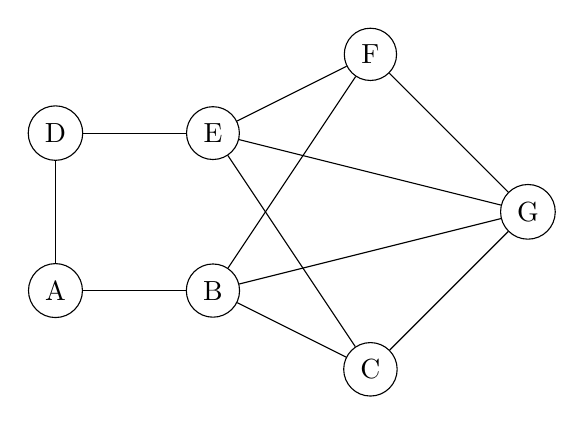
\begin{tikzpicture}[vertice/.style = {fill=white,circle,draw}]
\node[vertice] (A) at (0,0) {A};
\node[vertice] (B) at (2,0) {B};
\node[vertice] (C) at (4,-1) {C};
\node[vertice] (D) at (0,2) {D};
\node[vertice] (E) at (2,2) {E};
\node[vertice] (F) at (4,3) {F};
\node[vertice] (G) at (6,1) {G};

\draw (A) -- (B);
\draw (B) -- (C);
\draw (C) -- (G);
\draw (G) -- (F);
\draw (F) -- (E);
\draw (E) -- (D);
\draw (D) -- (A);
\draw (E) -- (C);
\draw (B) -- (F);
\draw (E) -- (G);
\draw (B) -- (G);
\end{tikzpicture} 
\end{center}
\end{ejer}

{\it Solución: }

% Escribe tu solución para el Ejercicio 5

No existe un camino euleriano cerrado en el grafo, ya que el nodo F y C es de grado impar.
Pero si abierto ya que solo F y C son impares.
Para calcularlo juntamos F y C

\begin{center}
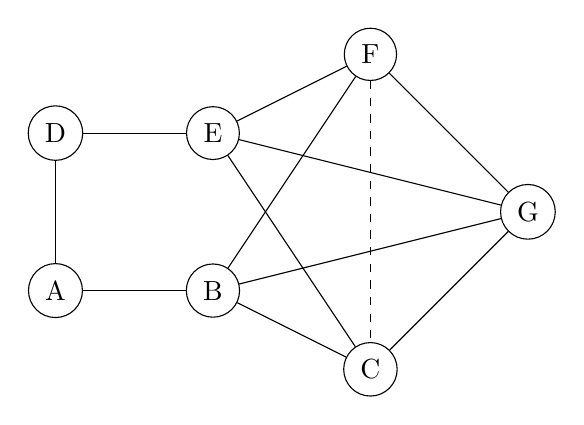
\begin{tikzpicture}[vertice/.style = {fill=white,circle,draw}]
	\node[vertice] (A) at (0,0) {A};
	\node[vertice] (B) at (2,0) {B};
	\node[vertice] (C) at (4,-1) {C};
	\node[vertice] (D) at (0,2) {D};
	\node[vertice] (E) at (2,2) {E};
	\node[vertice] (F) at (4,3) {F};
	\node[vertice] (G) at (6,1) {G};
	
	\draw (A) -- (B);
	\draw (B) -- (C);
	\draw (C) -- (G);
	\draw (G) -- (F);
	\draw (F) -- (E);
	\draw (E) -- (D);
	\draw (D) -- (A);
	\draw (E) -- (C);
	\draw (B) -- (F);
	\draw (E) -- (G);
	\draw (B) -- (G);
	\draw[dashed] (F) -- (C);
\end{tikzpicture} 
\end{center}

\begin{center}
	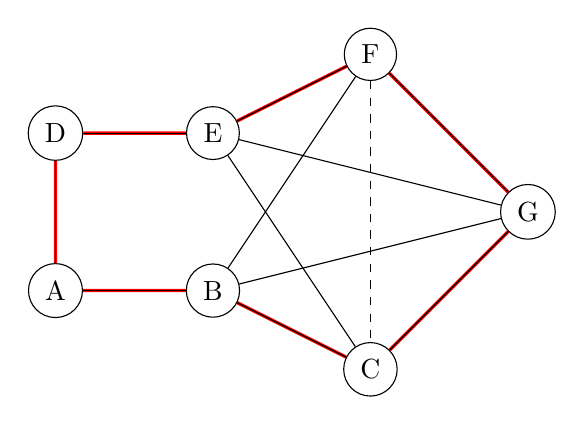
\begin{tikzpicture}[vertice/.style = {fill=white,circle,draw}]
		\node[vertice] (A) at (0,0) {A};
		\node[vertice] (B) at (2,0) {B};
		\node[vertice] (C) at (4,-1) {C};
		\node[vertice] (D) at (0,2) {D};
		\node[vertice] (E) at (2,2) {E};
		\node[vertice] (F) at (4,3) {F};
		\node[vertice] (G) at (6,1) {G};
		
		\draw[very thick, red] (A) -- (B) -- (C) -- (G) -- (F) -- (E) -- (D) -- (A);
		\draw (A) -- (B);
		\draw (B) -- (C);
		\draw (C) -- (G);
		\draw (G) -- (F);
		\draw (F) -- (E);
		\draw (E) -- (D);
		\draw (D) -- (A);
		\draw (E) -- (C);
		\draw (B) -- (F);
		\draw (E) -- (G);
		\draw (B) -- (G);
		\draw[dashed] (F) -- (C);
	\end{tikzpicture} 
\end{center}

$$
	{\color{red}(A) - (D) - (E) - (F) - (G) - (C) - (B)}
$$

\begin{center}
	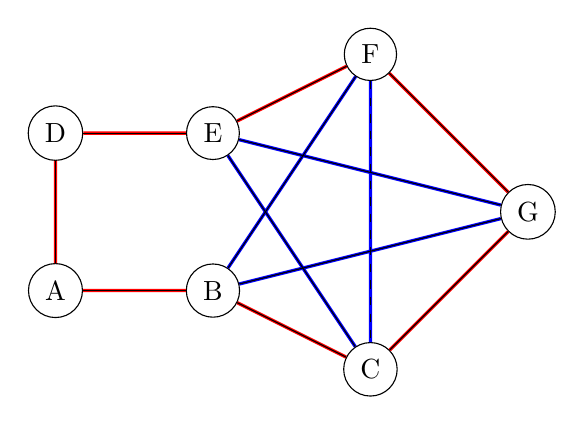
\begin{tikzpicture}[vertice/.style = {fill=white,circle,draw}]
		\node[vertice] (A) at (0,0) {A};
		\node[vertice] (B) at (2,0) {B};
		\node[vertice] (C) at (4,-1) {C};
		\node[vertice] (D) at (0,2) {D};
		\node[vertice] (E) at (2,2) {E};
		\node[vertice] (F) at (4,3) {F};
		\node[vertice] (G) at (6,1) {G};
		
		\draw[very thick, red] (A) -- (B) -- (C) -- (G) -- (F) -- (E) -- (D) -- (A);
		\draw[very thick, blue] (B) -- (G) -- (E) -- (C) -- (F) -- (B);
		\draw (A) -- (B);
		\draw (B) -- (C);
		\draw (C) -- (G);
		\draw (G) -- (F);
		\draw (F) -- (E);
		\draw (E) -- (D);
		\draw (D) -- (A);
		\draw (E) -- (C);
		\draw (B) -- (F);
		\draw (E) -- (G);
		\draw (B) -- (G);
		\draw[dashed] (F) -- (C);
	\end{tikzpicture} 
\end{center}

$$
	{\color{blue}(B) - (F) -- (C) - (E) - (G)}
$$

El circuito cerrado virtual
$$
	{\color{blue}(B) - (F) -- (C) - (E) - (G)}
$$

% Fin del ejercicio 5


\end{document}
